% DRG Predictor Paper — Hospital El Pino
% IEEE Conference Format, 6-page double-column
\documentclass[conference]{IEEEtran}

% ----- Packages -----
\usepackage[utf8]{inputenc}
\usepackage[T1]{fontenc}
\usepackage{graphicx}
\usepackage{booktabs}
\usepackage{amsmath}
\usepackage{amssymb}
\usepackage{hyperref}
\usepackage{cite}
\usepackage{xcolor}
\usepackage{multirow}
\usepackage{array}

% Figure paths
\graphicspath{{../figures/}{../}}

% Hyperref setup
\hypersetup{
    colorlinks=true,
    linkcolor=black,
    citecolor=blue,
    urlcolor=blue,
}

\begin{document}

% ----- Title -----
\title{Machine Learning Approaches for DRG Prediction\\from Clinical Coding Data: A Study of\\Hospital El Pino, Chile}

\author{
    \IEEEauthorblockN{Javier Far{\'\i}as, Uriel Navarrete, Fabiola Oses, Vicente Abarca}
    \IEEEauthorblockA{Universidad Andres Bello\\
    Santiago, Chile}
}

\maketitle

% ----- Abstract -----
\begin{abstract}
Diagnosis-Related Groups (DRGs) are the standard classification system for grouping hospital stays by clinical similarity and resource consumption. Accurate DRG assignment is critical for hospital reimbursement under Chile's FONASA public insurance system, which employs the IR-GRD v3.1 grouper. This paper presents a planned machine learning approach to predict the DRG assigned to a hospital stay from patient-level clinical data---specifically ICD-10 diagnoses, ICD-9-PCS procedures, patient age, and sex---using a dataset of 14,561 records from Hospital El Pino, a public facility in southern Santiago. We describe the dataset characteristics, propose a methodology encompassing preprocessing, candidate ML techniques (logistic regression, gradient-boosted trees, and a neural baseline), and evaluation metrics suited to the multi-class imbalanced classification setting. An exploratory data analysis reveals 526 distinct DRG classes, a heavily skewed class distribution dominated by obstetric categories, and a high-dimensional input space of 3,648 unique ICD-10 codes and 903 ICD-9-PCS procedure codes. This study lays the methodological groundwork for subsequent model development and evaluation.
\end{abstract}


% ----- Body -----
\section{Introduction}

Hospital reimbursement systems worldwide rely on Diagnosis-Related Groups (DRGs) to classify inpatient stays into clinically coherent categories with similar resource consumption profiles \cite{fetter1980drg}. In Chile, the public healthcare insurer FONASA adopted the IR-GRD v3.1 grouper to standardize billing across its network of public hospitals, linking reimbursement rates to the assigned DRG for each patient stay \cite{fonasa2016}. Accurate DRG assignment is thus a critical operational and financial concern for public hospitals.

The DRG grouping process maps a combination of clinical inputs---primary and secondary diagnoses coded in ICD-10 (CIE-10), procedures coded in ICD-9-PCS (CIE-9), patient age, and sex---to a single DRG class. Traditionally, this mapping is performed by rule-based grouper software that applies decision trees defined by the grouper vendor. However, the quality of DRG assignment depends heavily on the completeness and accuracy of the input codes, which are entered by clinical coders under time pressure and are susceptible to errors and omissions \cite{seroussi2017drg}.

Machine learning offers an alternative approach to DRG assignment. Rather than relying on hand-crafted decision rules, supervised ML models can learn the mapping from clinical inputs to DRG classes directly from historical data, potentially capturing patterns that rule-based systems miss. Several studies have demonstrated the feasibility of ML-based DRG prediction using structured clinical codes \cite{gartner2015ml, rajkomar2018scalable}, though most work has focused on US or European healthcare systems using CMS-DRG or G-DRG groupers.

The Chilean public health context presents a distinct setting. Hospital El Pino, located in the southern metropolitan area of Santiago, serves a predominantly low-income urban population and generates a volume of approximately 14,500 inpatient stays in the study period. The hospital's clinical coding practices, case mix, and the IR-GRD v3.1 grouper with FONASA 2016 pricing constitute a combination that has not been previously studied in the ML-for-DRG literature.

This paper presents the methodological groundwork for developing a DRG predictor for Hospital El Pino. Specifically, we (1)~describe the dataset and its characteristics, (2)~propose a preprocessing pipeline for the unordered sets of ICD codes, (3)~identify candidate ML techniques and justify their selection, (4)~define evaluation metrics appropriate for the multi-class imbalanced classification setting, and (5)~present an exploratory data analysis that characterizes the data quality, variable distributions, and class structure of the target DRG variable.

\section{Related Work}

The application of machine learning to DRG and clinical classification tasks has evolved across several related research streams.

\subsection{DRG Prediction from Structured Codes}

Early work by Fetter et al.\ established the DRG framework as a hierarchical classification of hospital stays based on principal diagnosis, procedures, age, and comorbidities \cite{fetter1980drg}. Subsequent studies explored statistical and ML approaches to automate or validate DRG assignment. Gartner et al.\ \cite{gartner2015ml} applied ensemble methods to predict DRGs from structured clinical codes, demonstrating that gradient-boosted trees outperformed rule-based groupers on incomplete coding data. More recently, Rajkomar et al.\ \cite{rajkomar2018scalable} showed that deep learning models could predict billing codes, including DRG-related outcomes, from electronic health records at scale, achieving strong performance on primary diagnosis and procedure prediction tasks.

\subsection{ICD Code Classification and Prediction}

A parallel stream of work addresses ICD code assignment from clinical free text, which is related but distinct from the DRG prediction task addressed here. Mullenbach et al.\ \cite{mullenbach2018caml} proposed Convolutional Attention for Multi-Label classification (CAML) to assign ICD codes from discharge summaries, establishing attention-based models as the state of the art for text-to-ICD prediction. Subsequent work by Vu et al.\ \cite{vu2020label} introduced label-aware attention mechanisms that further improved multi-label ICD classification on the MIMIC-III dataset \cite{johnson2016mimic}.

While these text-based approaches are not directly applicable to our structured-code input setting, they inform the broader landscape of clinical classification and demonstrate the feasibility of data-driven approaches to replace or augment rule-based clinical coding systems.

\subsection{Clinical Code Representations}

The representation of clinical codes as input features is a key methodological choice. Traditional approaches use multi-hot (bag-of-codes) encoding, where each code in the vocabulary is represented as a binary indicator. More sophisticated approaches learn dense embeddings of clinical codes from their co-occurrence patterns. Choi et al.\ \cite{choi2016med2vec} proposed Med2Vec to learn vector representations of medical codes from sequential clinical data, while Beam et al.\ \cite{beam2019clinical} demonstrated that clinical concept embeddings capture meaningful medical relationships.

Transformer-based models such as BEHRT \cite{li2020behrt} and Med-BERT \cite{rasmy2021medbert} extended the pre-training paradigm to clinical code sequences, learning contextualized representations from large-scale EHR data. However, these models typically require longitudinal patient trajectories across multiple visits, whereas our task considers a single inpatient stay with unordered code sets---a simpler but distinct problem formulation that favors bag-of-codes representations.

\subsection{Class Imbalance in Clinical Classification}

DRG classification is inherently imbalanced: a small number of DRGs account for the majority of hospital stays, while a long tail of rare DRGs may have very few examples. This mirrors the broader challenge of class imbalance in clinical ML, addressed through stratified sampling, class-weighted losses, and evaluation with macro-averaged metrics \cite{haixiang2017imbalanced, johnson2019survey}. Notably, interpolation-based oversampling methods such as SMOTE \cite{chawla2002smote} are ill-suited for high-dimensional binary feature spaces (such as multi-hot ICD codes), as interpolated samples do not correspond to valid code combinations.

\section{Objective}

The objective of this study is to develop a supervised machine learning model capable of predicting the Diagnosis-Related Group (DRG) assigned to a hospital stay, based on the patient's clinical coding data. Specifically, given an unordered set of up to 35 ICD-10 diagnoses, an unordered set of up to 30 ICD-9-PCS procedures, patient age (in years), and patient sex, the model will output a single predicted DRG class from the IR-GRD v3.1 classification system.

This constitutes a single-label, multi-class classification problem over approximately 526 distinct DRG classes observed in the Hospital El Pino dataset. The diagnosis and procedure inputs are treated as unordered sets---no clinical ordering is assumed among the coded entries. The study is scoped to a single hospital and does not require longitudinal patient history across multiple visits.

\section{Methodology}

\subsection{Dataset Description}

The dataset comprises 14,561 inpatient stay records from Hospital El Pino, a public hospital located in the southern metropolitan area of Santiago, Chile. Each record represents a single hospital stay and contains the following structured fields:

\begin{itemize}
    \item \textbf{Diagnoses}: 35 columns (1 principal + 34 secondary), each containing an ICD-10 (CIE-10) code with its Spanish-language description in the format \texttt{CODE - Description}. Unused slots are marked with a sentinel value ``\texttt{-}''.
    \item \textbf{Procedures}: 30 columns (1 principal + 29 secondary), each containing an ICD-9-PCS (CIE-9) procedure code with description, following the same format. Unused slots are similarly marked.
    \item \textbf{Patient age}: Numeric variable (age in years at time of admission), ranging from 0 to 121 years.
    \item \textbf{Patient sex}: Categorical variable (\textit{Hombre}/\textit{Mujer}; Male/Female).
    \item \textbf{DRG (target)}: The assigned DRG class from the IR-GRD v3.1 grouper with FONASA 2016 pricing, in the format \texttt{CODE - Description}.
\end{itemize}

Table~\ref{tab:dataset_overview} summarizes the key characteristics. The dataset contains 526 distinct DRG classes, 3,648 unique ICD-10 diagnosis codes, and 903 unique ICD-9-PCS procedure codes, reflecting considerable clinical diversity. The presence of ICD-10 code U07.1 (COVID-19) in the data indicates coverage of the pandemic period. The data is de-identified and provided for academic use.

\begin{table}[t]
\centering
\caption{Dataset Overview -- Hospital El Pino}
\label{tab:dataset_overview}
\begin{tabular}{lr}
\toprule
\textbf{Characteristic} & \textbf{Value} \\
\midrule
Total records (stays) & 14,561 \\
Diagnosis columns & 35 \\
Procedure columns & 30 \\
Unique DRG classes & 526 \\
Unique ICD-10 codes & 3,648 \\
Unique ICD-9-PCS codes & 903 \\
\midrule
Age (mean $\pm$ SD) & 39.4 $\pm$ 24.7 \\
Age (median) & 36 \\
Age range & 0--121 \\
Male / Female (\%) & 34.0 / 66.0 \\
\midrule
Diagnoses per stay (mean) & 7.2 \\
Diagnoses per stay (median) & 6 \\
Max diagnoses in a stay & 35 \\
Procedures per stay (mean) & 13.2 \\
Procedures per stay (median) & 11 \\
Max procedures in a stay & 30 \\
\bottomrule
\end{tabular}
\end{table}

\subsection{Preprocessing}

\subsubsection{Input Representation}
Since the diagnoses and procedures are explicitly unordered---the column position carries no clinical meaning---we will employ a \textbf{multi-hot (bag-of-codes)} encoding. Each record will be represented as a binary vector where each dimension corresponds to a code in the observed vocabulary: a 1 indicates the code is present in that stay, and a 0 indicates absence. Separate multi-hot vectors will be constructed for diagnosis codes and procedure codes, then concatenated with the numeric age and binary sex features.

This representation is preferred over padded-sequence encodings because (a)~it respects the unordered nature of the inputs, (b)~it is directly consumable by linear models and tree-based ensembles, and (c)~it avoids introducing spurious positional information that could mislead sequence-aware models.

\subsubsection{Sentinel Value Handling}
The sentinel value ``\texttt{-}'' is interpreted as ``slot not used,'' rather than as a missing value. In the multi-hot encoding, these entries simply do not activate any code dimension. The number of non-sentinel entries per stay is derived as a count feature (\texttt{n\_diagnoses}, \texttt{n\_procedures}).

\subsubsection{Feature Engineering}
Beyond the multi-hot code vectors, the following features will be derived:
\begin{itemize}
    \item \textbf{Age}: Retained as a continuous numeric variable.
    \item \textbf{Sex}: Encoded as a binary indicator (0/1).
    \item \textbf{Diagnosis count}: Number of non-empty diagnosis slots per stay.
    \item \textbf{Procedure count}: Number of non-empty procedure slots per stay.
\end{itemize}

\subsubsection{Vocabulary and Out-of-Vocabulary Policy}
The code vocabulary will be constructed from the training split. Codes appearing in validation or test sets but absent from training will be mapped to an \texttt{<UNK>} bucket, effectively ignored in the multi-hot vector. Codes will be validated against the CIE-10 and CIE-9 master catalogs provided with the dataset.

\subsection{Train/Validation/Test Split}

We will employ a stratified 70/15/15 split at the stay level, stratifying on the DRG class to ensure representation of rare classes across all partitions. Stratification is critical given the heavy class imbalance: without it, rare DRGs (with fewer than 10 examples) may be entirely absent from the validation or test sets, making evaluation unreliable.

\subsection{Machine Learning Techniques}

We propose three candidate model families, selected to span the spectrum from interpretable baselines to flexible nonlinear models:

\subsubsection{Logistic Regression (Baseline)}
A one-vs-rest (OvR) logistic regression classifier over the multi-hot feature space provides an interpretable linear baseline. Its coefficients reveal which codes are most predictive of each DRG, aiding clinical validation. Class weights will be set inversely proportional to class frequency to address imbalance. This baseline establishes the performance floor against which more complex models are measured.

\subsubsection{Gradient-Boosted Trees}
XGBoost or LightGBM with multi-class softmax loss represents the strong tabular-data baseline. Gradient-boosted trees handle sparse high-dimensional multi-hot inputs natively, tolerate class imbalance via the \texttt{scale\_pos\_weight} or \texttt{class\_weight} parameters, and require minimal feature engineering beyond the multi-hot encoding. Their ensemble structure captures nonlinear interactions between codes that logistic regression cannot model.

\subsubsection{Shallow Neural Network}
A feedforward neural network with 1--2 hidden layers (128--256 units, ReLU activation, dropout regularization) over the concatenated multi-hot input provides a feature-learning comparison. The network can discover dense representations of code patterns without requiring pre-trained embeddings. Class-weighted cross-entropy loss will be used for training.

We note that transformer-based clinical encoders (Med-BERT, BEHRT) are designed for longitudinal multi-visit sequences and are architecturally mismatched to our single-stay, unordered-set formulation. They are not included as candidates but are cited for context in Section~II.

\subsection{Evaluation Metrics}

Given the multi-class imbalanced nature of the DRG prediction task, we will evaluate models using the following metrics, each justified by a specific property of the problem:

\begin{itemize}
    \item \textbf{Top-1 Accuracy (Micro)}: The fraction of stays with correctly predicted DRG. This is the headline metric but is dominated by frequent classes and must not be reported alone.

    \item \textbf{Macro-Averaged F1}: Weights every DRG class equally. A model that excels on common DRGs but fails on rare ones will score well on accuracy but poorly on macro-F1, making this metric essential for evaluating rare-class performance.

    \item \textbf{Top-$k$ Accuracy ($k \in \{3, 5\}$)}: Measures whether the true DRG appears among the model's top-$k$ predictions. Operationally relevant because DRG assignment is often reviewed by a coder who can select from a shortlist.

    \item \textbf{Balanced Accuracy}: The macro-average of per-class recall. Directly interpretable as ``average recall across DRGs'' and a lighter-weight complement to macro-F1.

    \item \textbf{Per-Class Recall for Top-$N$ DRGs}: A per-class breakdown for the most frequent DRG classes, surfacing systematic confusions (e.g., between severity variants of the same base DRG) that aggregate metrics hide.

    \item \textbf{Matthews Correlation Coefficient (MCC)}: A single imbalance-aware scalar that accounts for all four confusion-matrix cells in the multi-class extension. Robust to extreme class skew.
\end{itemize}

We explicitly exclude ROC-AUC and PR-AUC, which are natural for binary tasks but awkward to interpret for single-label multi-class classification with hundreds of classes. SMOTE-style resampling is also excluded because interpolation in high-dimensional binary multi-hot space produces invalid code combinations; we rely instead on class-weighted losses and stratified sampling for imbalance mitigation.

\section{Exploratory Data Analysis}

\subsection{Data Quality}

The Hospital El Pino dataset exhibits high completeness for the core variables: age, sex, and DRG target are present for all 14,561 records (100\% completeness). The 35 diagnosis and 30 procedure columns use the sentinel value ``\texttt{-}'' to indicate unused slots, which is a structural feature of the fixed-width column layout rather than true data missingness.

\begin{table}[t]
\centering
\caption{Sentinel Value (``-'') Summary Across Code Columns}
\label{tab:missingness}
\begin{tabular}{lr}
\toprule
\textbf{Metric} & \textbf{Value} \\
\midrule
Total code cells (65 columns $\times$ N) & 946,465 \\
Cells with data (non-sentinel) & 296,920 (31.4\%) \\
Empty cells (sentinel ``-'') & 649,545 (68.6\%) \\
\midrule
Age column completeness & 100.0\% \\
Sex column completeness & 100.0\% \\
DRG target completeness & 100.0\% \\
\bottomrule
\end{tabular}
\end{table}

As shown in Table~\ref{tab:missingness}, 68.6\% of the 946,465 total code cells (65 columns $\times$ 14,561 records) contain the sentinel value, reflecting the fact that most stays have far fewer diagnoses and procedures than the maximum slot capacity. Fig.~\ref{fig:completeness} visualizes the completeness by column position: the principal diagnosis (slot~1) is populated for 100\% of records, with completeness declining steeply for secondary slots. A similar pattern holds for procedure columns, where the principal procedure is present in the majority of records but higher-numbered slots are increasingly sparse.

\begin{figure}[t]
    \centering
    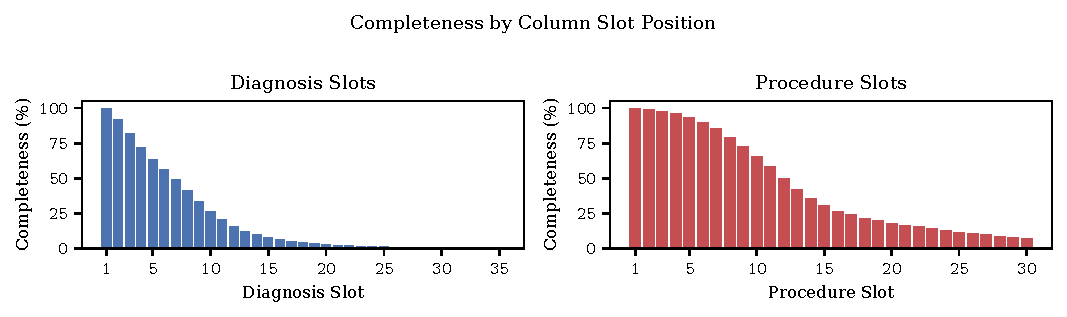
\includegraphics[width=\columnwidth]{fig_completeness.pdf}
    \caption{Completeness rates by column slot position for diagnosis (left) and procedure (right) columns. Slot~1 (principal) is fully populated; secondary slots decline sharply.}
    \label{fig:completeness}
\end{figure}

An age value of 121 years was observed, which may represent a data-entry error or a coded value for undetermined age. Further validation against hospital records would be needed to confirm; for the purposes of this study, the value is retained as-is.

\subsection{Descriptive Statistics}

\begin{table}[t]
\centering
\caption{Age Distribution by Sex}
\label{tab:age_summary}
\scriptsize
\begin{tabular}{@{}lrrrrrrrr@{}}
\toprule
\textbf{Sex} & \textbf{N} & \textbf{Mean} & \textbf{SD} & \textbf{Min} & \textbf{Q1} & \textbf{Med.} & \textbf{Q3} & \textbf{Max} \\
\midrule
    Male & 4,944 & 43.6 & 28.2 & 0 & 19 & 51 & 66 & 97 \\
    Female & 9,617 & 37.3 & 22.4 & 0 & 24 & 33 & 52 & 121 \\
    Overall & 14,561 & 39.4 & 24.7 & 0 & 23 & 36 & 60 & 121 \\
\bottomrule
\end{tabular}
\end{table}

Table~\ref{tab:age_summary} presents the age distribution by sex. The overall mean age is 39.4 years (SD = 24.7), with a median of 36 years. The dataset is 66.0\% female and 34.0\% male, reflecting the dominance of obstetric DRGs (cesarean sections and vaginal deliveries) in the case mix. Female patients have a lower mean age (35.6 years) compared to male patients (47.0 years), consistent with the inclusion of a substantial population of childbearing-age women.

On average, each stay has 7.2 diagnoses (median 6, max 35) and 13.2 procedures (median 11, max 30), indicating that the typical clinical record carries a moderate coding density with high variability.

\subsection{Visualizations}

\subsubsection{DRG Class Distribution}

\begin{figure}[t]
    \centering
    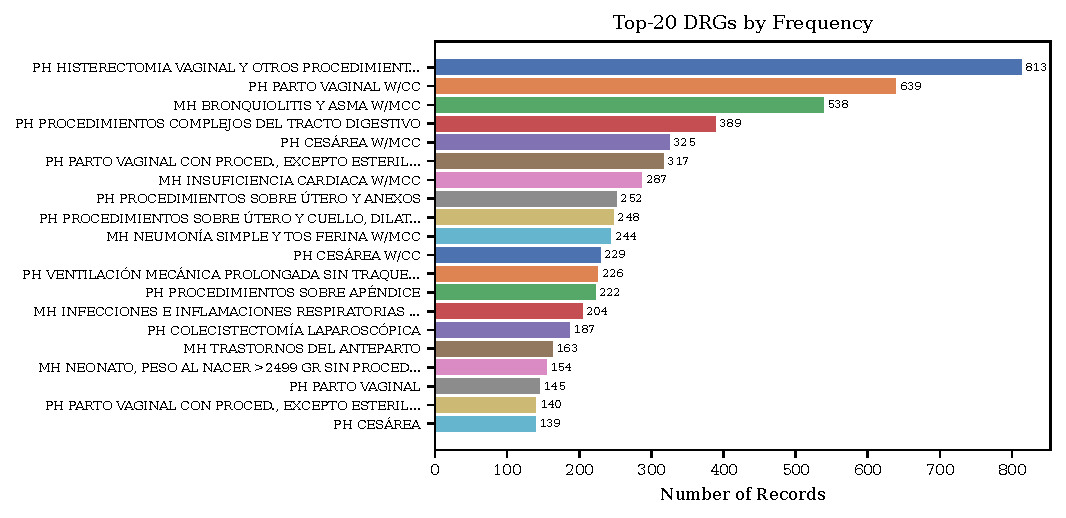
\includegraphics[width=\columnwidth]{fig_drg_top20.pdf}
    \caption{Top-20 DRGs by frequency. Obstetric categories (cesarean section, vaginal delivery) dominate the case mix.}
    \label{fig:drg_top20}
\end{figure}

Fig.~\ref{fig:drg_top20} shows the top-20 DRGs by frequency. The distribution is heavily skewed: the top DRG (cesarean section) accounts for 5.6\% of all records, and the top-5 DRGs collectively cover 18.6\% of the dataset. The long tail is substantial---of the 526 distinct DRG classes, many have fewer than 10 occurrences. This extreme imbalance motivates the use of macro-averaged metrics and class-weighted losses described in Section~IV-E.

\begin{table}[t]
\centering
\caption{Top-10 DRGs by Frequency}
\label{tab:top_drgs}
\scriptsize
\begin{tabular}{p{4.2cm}rrr}
\toprule
\textbf{DRG Description} & \textbf{Count} & \textbf{\%} & \textbf{Cum.\%} \\
\midrule
    PH CESÁREA & 813 & 5.6 & 5.6 \\
    PH PARTO VAGINAL CON PROCED., EXCEP... & 639 & 4.4 & 10.0 \\
    PH PARTO VAGINAL & 538 & 3.7 & 13.7 \\
    MH NEONATO, PESO AL NACER {>}2499 GR ... & 389 & 2.7 & 16.3 \\
    MH TRASTORNOS DEL ANTEPARTO & 325 & 2.2 & 18.6 \\
    PH COLECISTECTOMÍA LAPAROSCÓPICA & 317 & 2.2 & 20.7 \\
    MH INFECCIONES E INFLAMACIONES RESP... & 287 & 2.0 & 22.7 \\
    PH PROCEDIMIENTOS SOBRE APÉNDICE & 252 & 1.7 & 24.4 \\
    PH VENTILACIÓN MECÁNICA PROLONGADA ... & 248 & 1.7 & 26.2 \\
    PH CESÁREA W/CC & 244 & 1.7 & 27.8 \\
\bottomrule
\end{tabular}
\end{table}

\subsubsection{Age Distribution by Sex}

\begin{figure}[t]
    \centering
    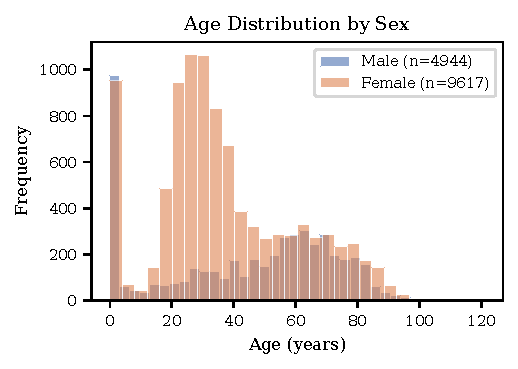
\includegraphics[width=\columnwidth]{fig_age_hist_by_sex.pdf}
    \caption{Age distribution by sex. The female distribution shows a pronounced peak in the 20--35 age range, driven by obstetric admissions.}
    \label{fig:age_by_sex}
\end{figure}

Fig.~\ref{fig:age_by_sex} presents overlaid histograms of age by sex. The female distribution exhibits a bimodal pattern with a pronounced peak in the 20--35 age range (corresponding to childbirth-related admissions) and a secondary peak in the elderly population. The male distribution is more uniformly spread across adult ages with a higher concentration in the 50--80 range.

\subsubsection{Diagnosis and Procedure Count Distributions}

\begin{figure}[t]
    \centering
    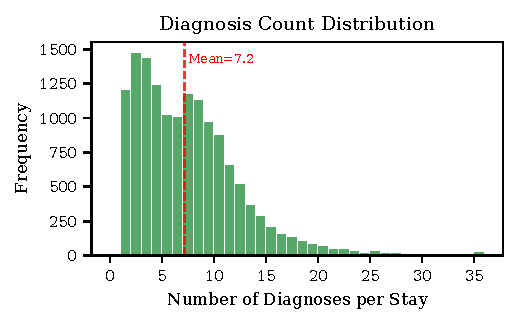
\includegraphics[width=\columnwidth]{fig_diag_count_dist.pdf}
    \caption{Distribution of the number of diagnoses per hospital stay.}
    \label{fig:diag_count}
\end{figure}

\begin{figure}[t]
    \centering
    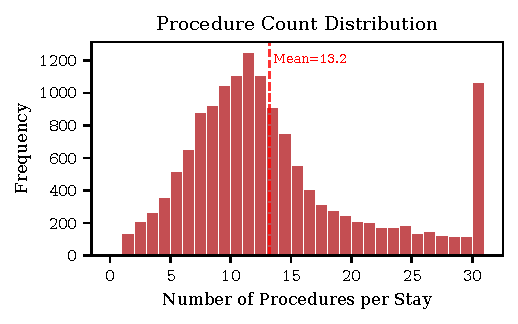
\includegraphics[width=\columnwidth]{fig_proc_count_dist.pdf}
    \caption{Distribution of the number of procedures per hospital stay.}
    \label{fig:proc_count}
\end{figure}

Fig.~\ref{fig:diag_count} shows the diagnosis-count distribution: the majority of stays have between 3 and 12 diagnoses, with a right-skewed tail extending to the maximum of 35. Fig.~\ref{fig:proc_count} shows the analogous distribution for procedures, where the typical stay has 5--20 procedures. These distributions inform the multi-hot encoding choice: the high variability in code counts makes fixed-length representations suboptimal, while the bag-of-codes approach naturally accommodates variable-length inputs.

\subsubsection{Top Principal Diagnoses and Procedures}

\begin{figure*}[t]
    \centering
    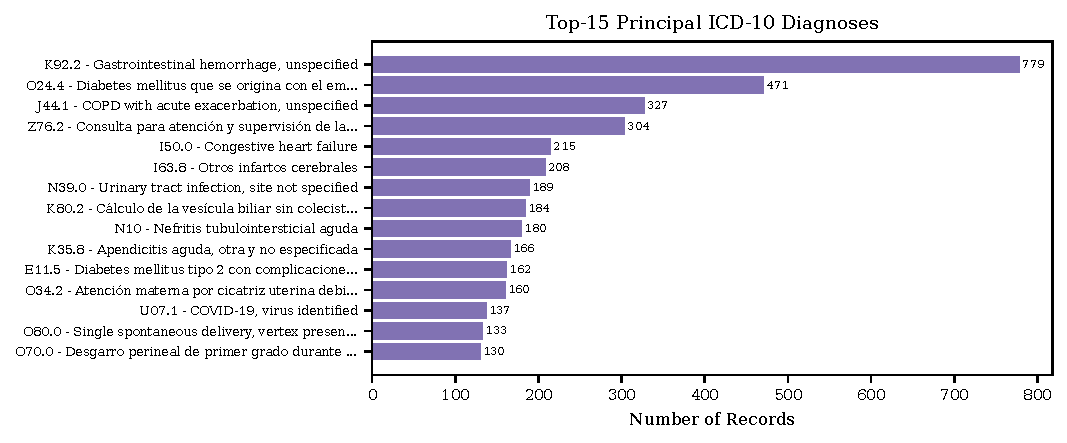
\includegraphics[width=\textwidth]{fig_top_icd10_principal.pdf}
    \caption{Top-15 principal ICD-10 diagnoses. Septicemia, heart failure, pneumonia, and obstetric conditions are the most frequent.}
    \label{fig:top_icd10}
\end{figure*}

\begin{figure*}[t]
    \centering
    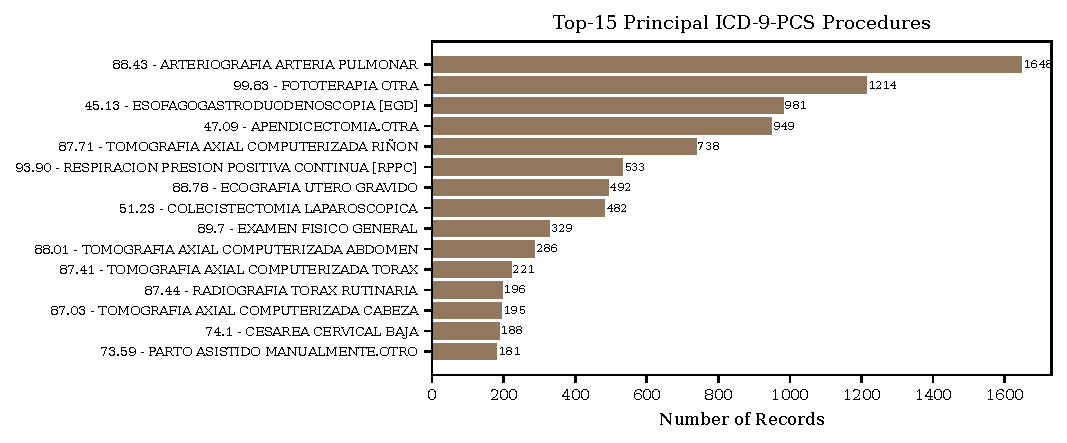
\includegraphics[width=\textwidth]{fig_top_icd9_principal.pdf}
    \caption{Top-15 principal ICD-9-PCS procedures. Cesarean sections and vaginal deliveries are the most common procedures, consistent with the DRG distribution.}
    \label{fig:top_icd9}
\end{figure*}

Fig.~\ref{fig:top_icd10} and Fig.~\ref{fig:top_icd9} display the top-15 principal diagnoses and procedures, respectively. The principal diagnoses are led by septicemia (A41.8), congestive heart failure (I50.0), and unspecified pneumonia (J18.9)---common conditions for a general public hospital. Notably, COVID-19 (U07.1) appears among the frequent diagnoses, confirming coverage of the pandemic period. The principal procedures are dominated by obstetric interventions (cesarean sections, vaginal deliveries) and general surgical procedures (appendectomy, cholecystectomy), reflecting the hospital's role as a community facility serving both obstetric and general medical populations.


% ----- References -----
\bibliographystyle{IEEEtran}
\bibliography{../references/refs}

\end{document}
